\documentclass[tikz]{standalone}
\usetikzlibrary{positioning}

\newcommand{\po}[2]{\draw [->, thick] (#1) to node[above] {\Large{so}} (#2);}
\newcommand{\povis}[2]{\draw [->, thick] (#1) to node[above] {\Large{so}$,$ \Large{vis}} (#2);}
%p\newcommand{\povis}[2]{\draw [->, thick] (#1) to node[above] {\Large{so}} node[below] {\Large{vis}} (#2);}
\newcommand{\vis}[2]{\draw [->, thick, dashed] (#1) to node[above, sloped, near end] {\Large{vis}} (#2);}
\newcommand{\ar}[2]{\draw [->, thick, dotted] (#1) to node[above, sloped] {\Large{ar}} (#2);}
\newcommand{\vvis}[2]{\draw [->, thick, dashed, allow upside down] (#1) to node[above, sloped] {\Large{vis}} (#2);}

\begin{document}
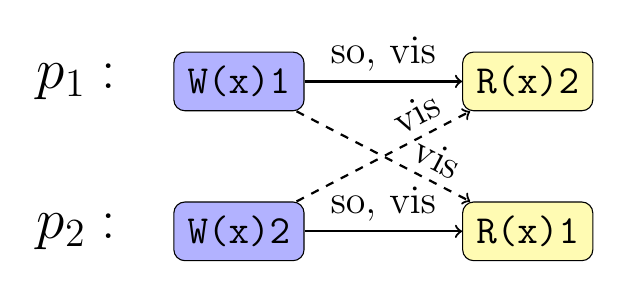
\begin{tikzpicture}
\tikzset{
  wop/.style = {rectangle, rounded corners, fill = blue!30, draw, font = \Large, inner sep = 5pt},
  rop/.style = {rectangle, rounded corners, fill = yellow!30, draw, font = \Large, inner sep = 5pt}, process/.style = {font = \huge},
  %po/.style = {->, very thick},
  rw/.style = {->, shorten >= 3pt, very thick, dashed},
  %vis/.style = {->, shorten >= 3pt, very thick, dashed}
}

  \node (p1) [process] {$p_1:$};
  \node (wx1) [wop, right = 0.6cm of p1] {\texttt{W(x)1}};
  \node (rx2) [rop, right = 2cm of wx1] {\texttt{R(x)2}};

  \node (p2) [process, below = 1.2cm of p1] {$p_2:$};
  \node (wx2) [wop, right = 0.6cm of p2] {\texttt{W(x)2}};
  \node (rx1) [rop, right = 2cm of wx2] {\texttt{R(x)1}};

  \povis{wx1}{rx2};
  \povis{wx2}{rx1};

  \vis{wx1}{rx1};
  \vis{wx2}{rx2};

\end{tikzpicture}
\end{document}
